% GigBid R&D report (AI-4016). Build: cd docs/report && pdflatex main && pdflatex main
% Tables in tables/ are generated by `python -m scripts.make_report_tables` from evals/results/. \pending{} marks
% text that depends on results still to be measured; the final build must contain none.
\documentclass[10pt,a4paper]{article}
\usepackage[margin=2cm]{geometry}
\usepackage[T1]{fontenc}
\usepackage{lmodern,microtype,booktabs,graphicx,xcolor,enumitem}
\usepackage[hidelinks]{hyperref}
\setlist{nosep,leftmargin=1.2em}
\setlength{\parskip}{3pt}
\setlength{\emergencystretch}{2em}
\newcommand{\pending}[1]{\textcolor{red}{[#1]}}
\newcommand{\file}[1]{\texttt{\small #1}}
\newcommand{\tablefrom}[2]{\begin{table}[h]\centering\caption{#2}\input{tables/#1}\end{table}}

\title{\textbf{GigBid: a multi-agent freelancer copilot}\\[2pt]\large AI-4016 R\&D report, engineering design review}
\author{Mushahid Hussain (23I-0541), FAST-NUCES Islamabad}
\date{November 2026}

\begin{document}
\maketitle
\vspace{-1em}
\noindent Every measured result in this report is read from a file in \file{evals/results/} (or an archived run or
commit named next to it), and every claim points to a file, a trace or a commit in the repository
(\url{https://github.com/mushi-PMA/gigbid}). Most samples are small; we give $n$ wherever it matters.

% ------------------------------------------------------------------------------------------------------------------
\section{Problem and constraints}
A freelancer spends hours scanning job feeds, spends paid Connects on jobs they are unlikely to win, sends generic
proposals and meets scams that ask for free work or off-platform payment. GigBid automates discovery, assessment and
drafting; the freelancer keeps every decision.

\textbf{What must never be automated.} Submitting a proposal, sending a message and spending Connects always wait for
the freelancer's approval in the web UI (LangGraph \texttt{interrupt()}); in live mode Upwork asks again. A per-user
autonomy setting may auto-skip low-fit jobs; it can never send. GigBid never claims experience the portfolio does
not show, never moves contact or payment off the platform, and never scrapes or automates a website.

\textbf{Budgets} (declared in \file{agent/config.yaml} before the holdout run): p95 latency 20\,s per job analysed
and 90\,s per proposal; US\$0.002 per job analysed and US\$0.01 per proposal on the open profile.

% ------------------------------------------------------------------------------------------------------------------
\section{Architecture}
\begin{figure}[h]\centering
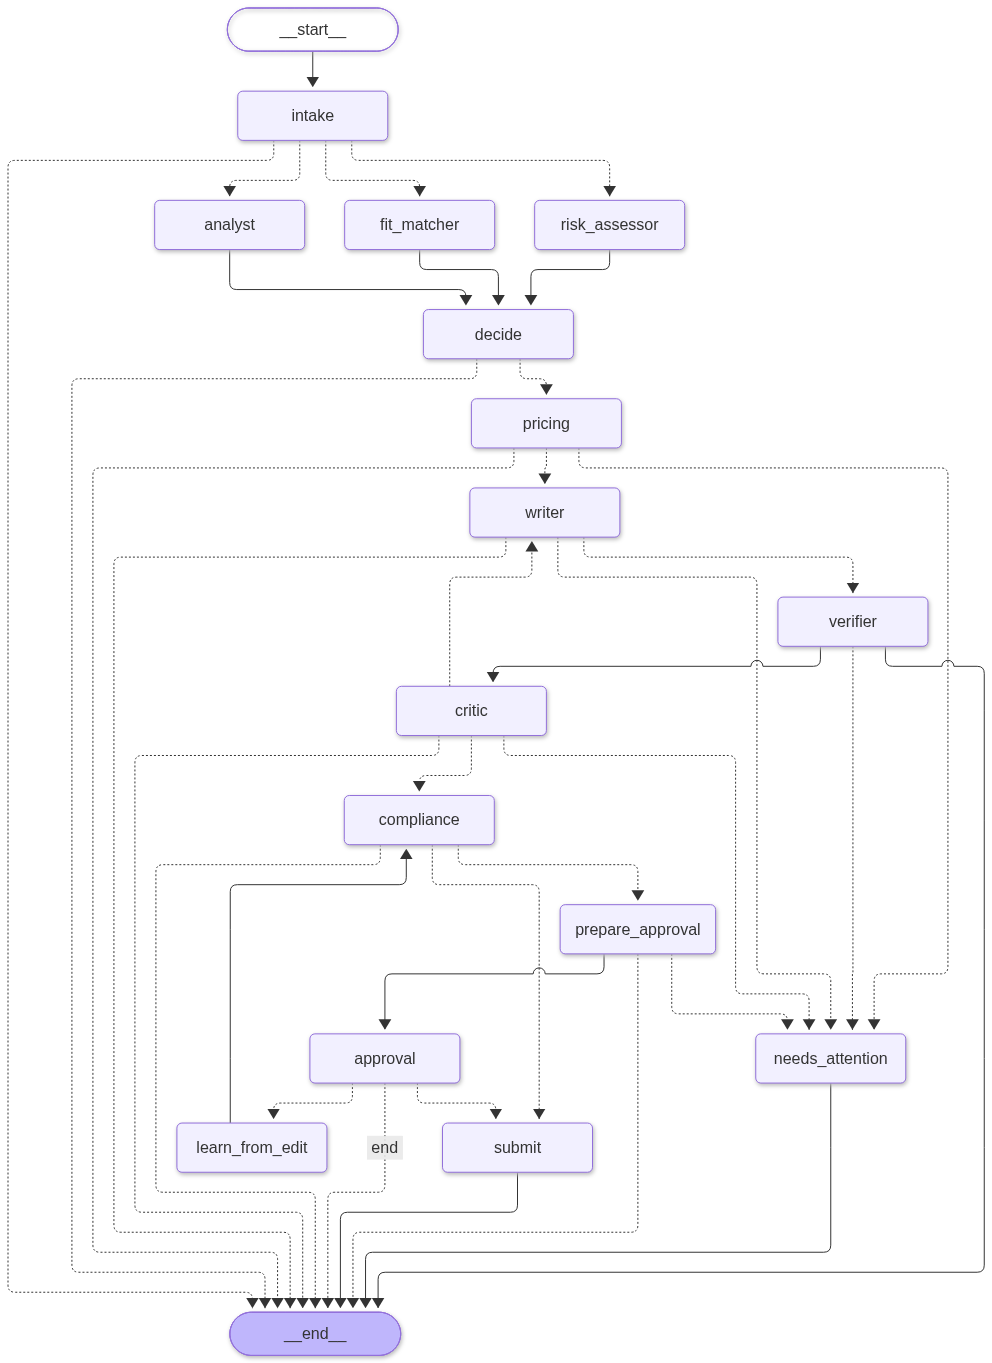
\includegraphics[height=8.4cm]{../images/bid_graph.png}\hspace{1em}
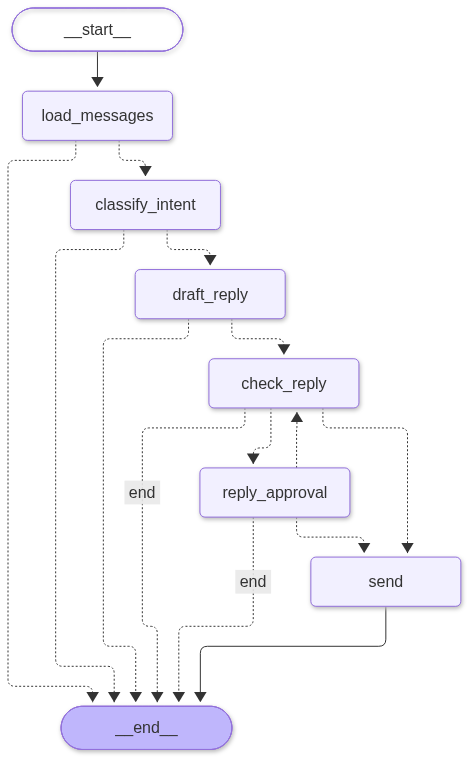
\includegraphics[height=5.2cm]{../images/conversation_graph.png}
\caption{The bid graph (left) and the conversation graph (right), rendered from code (\file{make graphs}).}
\end{figure}

\textbf{Bid graph} (one thread per job). The Scout hands a job in; the Job Analyst, Risk Assessor and Fit Matcher run
in parallel (\texttt{Send}); a deterministic decision node chooses skip, watch or bid with reasons; the Pricing
Strategist, Proposal Writer, claim verification, Critic (at most two send-backs) and Compliance Guard follow; the
graph interrupts with a dry-run preview before anything is sent, and submits exactly once. \textbf{Conversation graph}
(one thread per client conversation): load messages, classify intent, draft a reply or interview slots, check
compliance, interrupt for approval, send.

\textbf{Marketplace port.} One interface (\file{agent/marketplace\_port.py}) over the Marketplace MCP server, which
routes to a GigSim adapter or a live Upwork adapter (official Upwork MCP server, OAuth 2.1, tokens encrypted per
user) by configuration. The graph cannot tell which marketplace it uses.

\textbf{MCP surface.} Three servers built with the official SDK: Portfolio (read: \texttt{search\_evidence},
\texttt{get\_case\_study}, \texttt{list\_skills}, resources and prompts), Marketplace (reads plus
\texttt{create\_proposal\_draft}, \texttt{submit\_proposal}, \texttt{send\_message} with Pydantic schemas, output
schemas, annotations, idempotency keys and \texttt{dry\_run}) and Workspace (free slots, interview holds, email
drafts). Third-party: Upwork's official server and GitHub's official server (repo ingestion). Each agent receives
only the tools on its allowlist. Writes need an \emph{approval token} that signs the exact payload the human approved,
so nothing the human did not see can be sent (ADR 0005). Every call is audited (append-only table).

\textbf{State, trace and memory are kept apart.} Typed state holds what one job needs now, with reducers where
parallel branches write. The execution trace (every tool call, argument, result, tokens and cost per node) goes to
Phoenix and the audit log. Long-term memory holds only promoted knowledge: a style rule enters only after the same
edit pattern appears in two separate approvals, and an outcome summary only after three resolved proposals in a
category (\file{agent/memory/promotion\_rules.py}).

\textbf{Why each agent exists.} The Analyst, Risk Assessor and Fit Matcher need different inputs and tools and are
independent, so they run in parallel and a strong fit can never hide a risk flag. Pricing has hard rules (the floor,
the Connects budget). The Writer gets the strongest model; claim verification and the Critic check it
independently; the Compliance Guard applies the policy pack, which lives in configuration.

% ------------------------------------------------------------------------------------------------------------------
\section{R\&D question A: tool granularity}
\textbf{Hypothesis} (pre-registered in \file{docs/HYPOTHESES.md}): our 10-tool set with rewritten descriptions beats
an 18-tool fine-grained set and a 3-tool coarse set on selection and argument accuracy; the coarse set uses the fewest
tokens. \textbf{Setup.} 40 tasks with known correct calls (4 per capability, ids taken from GigSim and the personas,
\file{evals/datasets/tool\_tasks.json}); one tool-calling turn per task with native tool use, same model and system
prompt for all three sets (\file{evals/runners/tool\_granularity.py}).
\tablefrom{tools}{Tool-design study on 40 tasks.}
\textbf{Conclusion.} H-A is supported: our set is the most accurate, and, as predicted, the coarse set uses the fewest
tokens. Our 10 tools picked the
right tool on all 40 tasks and filled the arguments right on 39 (97.5\%); the 18-tool set scored 95\% and 92.5\%, the
3-tool set 95\% and 77.5\%. The coarse set is the cheapest (372 tokens per task) but loses on arguments: one tool
with an \texttt{action} field makes the model guess nested parameters (pricing category, job id, evidence filters).
The fine set fails where two tools overlap (\texttt{get\_hourly\_rate\_stats} against market pricing, case-study
search against skill listing). Our set costs the most tokens per task (1,116), because the rewritten descriptions
say when to use each tool and when not to; that text is what removes the overlaps, so we keep it.

% ------------------------------------------------------------------------------------------------------------------
\section{R\&D question B: retrieval, claim verification and what ships}
The persona corpora are built to defeat naive retrieval: code and prose mixed, each project described up to three
ways (case study, README, past proposals), skills implied, and proposals whose outcome matters more than their
wording. We implemented V0 to V8 as configurable components (\file{rag/variants/}), each taken from published work:
dense retrieval as in RAG~\cite{lewis2020rag}, BM25 and dense lists merged by reciprocal rank fusion~\cite{cormack2009rrf}
(V2), a cross-encoder reranker~\cite{nogueira2019rerank} (V3), HyDE~\cite{gao2023hyde} (V7) and corrective
retrieval~\cite{yan2024crag} (V8); the retriever composes them from a string such as \texttt{v1+v2+v3+v5}. Claim
verification checks each atomic claim against the evidence, in the spirit of FActScore~\cite{min2023factscore}. An evidence item is a portfolio project: retrieving its case study, README,
code or proposal counts as finding it. Hypotheses: V1+V2+V3 raises Recall@5 by 10 points on jobs with four or more
requirements (H-B1); V2 beats V0 for every persona (H-B2); claim verification halves unsupported claims (H-B4: met narrowly, 2.13 to 1.00 per proposal on 8 letters).
\tablefrom{rag}{Retrieval variants on the dev set.}
\tablefrom{main}{Baseline V0 against the shipped pipeline.}
\tablefrom{claims}{Unsupported claims before and after claim verification (shipped pipeline).}
\textbf{Judge calibration.} A model judge can be biased toward length and style~\cite{zheng2023judge}, so the rubric
judge was compared with my own blind labels on 30 proposals (Cohen's kappa~\cite{cohen1960kappa}):
agreement was poor, with Cohen's kappa 0.01 and quadratic-weighted kappa 0.29; 7 of 30 scores matched exactly and 19
were within one point (\file{evals/results/judge\_calibration.json}). The judge was kinder than me (mean 3.70 against
2.63) and gave 4 to 24 of the 30 letters, so it hardly separates strong letters from weak ones. Two disagreements: for
a senior Azure data engineer post (item 16) the judge gave 3 and I gave 1, because the letter never mentions Azure,
Data Factory or Databricks; I was right, as the judge does not punish a missing core requirement. For the contract
report job (item 24) I gave 2 because the letter seemed to invent the client's CTO and GM, but the full post does name
them and my labelling sheet showed only its first 1,500 characters, so the judge was right. Small judge-score gaps in
this report (3.57 against 3.63, 3.88 against 3.75) should therefore not be read as quality differences.
The blind pairwise human panel (classmates choose between anonymised V0 and shipped proposals for the same job,
\file{evals/runners/human\_panel.py}) is prepared on the 5 jobs both pipelines drafted, but had not been rated when
this report was written; with 5 pairs it could only show a very large preference.
\textbf{Ablation and breakdown.} Removing hybrid search (V2) costs 0.062 nDCG@10 and removing the outcome boost (V4)
0.021 (\file{evals/results/ablation.json}), so both earn their place and V2 matters most. The breakdown is the honest
part: the shipped retrieval helps the web-developer persona most (nDCG@10 0.518 to 0.630) and e-commerce and data-pipeline
jobs, but it is worse than V0 for the AI/ML persona (0.610 to 0.584; V2 alone 0.604) and much worse on LLM-app jobs (Recall@5 0.582 to
0.154, only 6 jobs), which is why H-B2 (``V2 beats V0 for every persona'') is refuted. H-B1 is refuted too: on the 29 jobs with four or
more requirements that both runs share, V1+V2+V3 reached Recall@5 0.368 against 0.432 for V0, a drop of six points
where we predicted a gain of ten (rows of \file{rag\_variants\_model.json} and \file{rag\_variants\_offline.json}).
\tablefrom{ablation}{The shipped retrieval with one component removed at a time (dev set, no model calls).}
\tablefrom{breakdown}{V0 against the shipped retrieval by persona, number of requirements and job type (dev set).}
\textbf{Where better retrieval did not raise replies.} The shipped retrieval beats V0 on nDCG@10 (0.597 against 0.566 on
the same 150 jobs), yet in GigSim V0's proposals did as well: every one of V0's 7 drafted proposals got a reply, against
7 of the shipped pipeline's 8, with judge scores of 3.57 and 3.63 (\file{evals/results/proposals\_v0.json},
\file{proposals\_best.json}; the two pipelines drafted overlapping but not identical sets of the 12 jobs, so these
rates are not paired). H-B3 (better retrieval raises the reply rate) is not supported. A likely reason is in how GigSim's clients score a letter
(\file{gigsim/clients.py}): naming the job's skills, reusing the post's own words, the price, avoiding a generic opening
and answering screening questions. Which evidence a letter cites is not scored, so better retrieval can only help
through those, and both pipelines use the same Writer, which is told to open with the client's problem in their own
terms. The shipped pipeline's letters also carried a higher share of unsupported claims after verification (22\%
against 16\%; 1.00 against 0.86 per proposal); the verifier flagged fewer claims in V0's letters to begin with and
removed none of them (0.86 before and after), which we did not investigate further. With 7 and 8 proposals none of these differences is significant, so the
shipped choice rests on retrieval quality and cost, not on replies.
\textbf{What ships.} V2+V4 (hybrid BM25 and dense search with the outcome-aware boost, \file{docs/adr/0003-rag-variant.md}).
V2+V4+V7 retrieved better (nDCG@10 0.629 against 0.587 on the same 60 jobs, \file{evals/results/rag\_variants\_model.json}),
but HyDE adds a model call to every search and the binding limit on our free tier is tokens per day per key, not
dollars; V2+V4 adds no model call and gives up about 0.04 nDCG@10. The corrective loop (V8) lifted plain hybrid search
a little on 30 dev jobs (nDCG@10 0.558 against 0.530 for V2 on the same jobs) but stayed below V2+V4 (0.612) and
took 21.7\,s per search on average (\file{rag\_variants\_model\_late.json}); V6 was not run within the token budget. The cross-encoder (V3) was dropped because it lowered nDCG@10 on every
combination and was slow on CPU (p95 retrieval 17.7\,s for V2+V3 against 4.7\,s for V2+V4,
\file{rag\_variants\_offline.json}). Claim verification ships on: in the shipped
proposal study it cut unsupported claims from 2.13 to 1.00 per proposal (47\% to 22\% of claims,
\file{evals/results/proposals\_best.json}). The cost is real: 44,238 tokens and \$0.0102 per drafted proposal (with the
Critic stop that ships, the same 8 drafts cost \$0.0092 and kept 0.63 unsupported claims each,
\file{proposals\_best\_critic\_stop.json}), and on four
of twelve forced weak-fit jobs verification removed so many sentences that the Critic loop ran out of token budget and
the job went to a human instead (\file{docs/FAILURES.md}, row 13).

% ------------------------------------------------------------------------------------------------------------------
\section{R\&D question C: single agent, prebuilt supervisor, or our graph}
On 9 fixed dev jobs (3 per persona; reduced from 50, see the deviation in \file{docs/HYPOTHESES.md}) we compare (a) one ReAct~\cite{yao2023react} agent holding all tools, (b) \texttt{langgraph-}\linebreak[0]\texttt{supervisor} with three
tool-using workers and (c) the hand-built graph, with the same MCP tools, model family, verifier and simulated
clients (\file{evals/runners/architecture\_comparison.py}). Hypothesis H-C: (c) wins on accuracy, unsupported claims
and violations; (a) is cheapest and can tie on simple, clearly relevant jobs.
\tablefrom{architectures}{Architecture comparison on 9 dev jobs.}
\textbf{Result} (\file{evals/results/architecture\_comparison.json}). H-C is refuted on decisions and only weakly
supported on grounding. The prebuilt supervisor had the best bid-or-skip accuracy (0.667, against 0.556 for one agent
and 0.444 for our graph), but its proposals carried 6.0 unsupported claims each and one policy violation reached its
final text; the single agent's carried 2.0; ours 0.5, with no violation. These grounding numbers rest on 3, 2 and 2
letters, each design drafting only the jobs it chose to bid on; where two designs drafted the same job the order holds
(dev-aiml-0003: supervisor 7, graph 1; dev-web-0003: supervisor 5, single agent 3), but this is a direction, not a
measured gap. The graph's calls were replayed from the cache while the baselines ran live. Our graph is also the most expensive: 23,651 tokens per job
against 8,446 and 7,448, because three agents read every job in parallel and the Writer, verifier and Critic loop over
each draft. Its lower accuracy has the causes found in the failure analysis: three gold bids were not bid on (the extractor
splitting named tools into extra requirements, rows 8 and 9, and the unverified-client rule, row 10) and two posts with
low skill overlap were bid on (the matcher crediting nearby skills, rows 6 and 7).
\textbf{Where (a) and (b) win and would we ship them.} Both are three times cheaper per job, and on these nine jobs
both decide better; nine jobs is too few to call that difference reliable. We would still ship the graph: the cost of a wrong decision is one
watched job, while an unsupported claim sent to a client is the failure the brief (R5) and the platform punish. The
cheaper fix is to keep the graph and loosen the client rule, not to drop verification. Latency is not compared: the
graph's calls in this run were replayed from the evaluation cache, which takes no time (Section~\ref{sec:holdout}).

% ------------------------------------------------------------------------------------------------------------------
\section{The change request}
On 2 November 2026 GigSim's policy moved to v2: premium jobs (fixed budget at least \$1,000 or hourly at least \$50)
cost 4 extra Connects, and proposals must not contain links. Because rules, detection patterns and Connects pricing
live in \file{data/policy\_pack/policy.yaml}, the change was a data edit: \textbf{13 lines added and 4 removed in two
policy files, zero lines of Python}, plus a test proving our Connects cost now equals GigSim's and that the cleaned
text passes GigSim's v2 check. It took about 15 minutes. The lesson: rule-shaped changes are cheap with this design;
a change that needs new logic (for example a per-client proposal limit) would need code in the Pricing Strategist
(\file{docs/CHANGE\_REQUEST.md}).

% ------------------------------------------------------------------------------------------------------------------
\section{Signature extension: proposal experiments (X2)}
The Writer's strategy is configuration (\texttt{writer.strategy}). Strategy A opens with the client's problem and the
most relevant evidence; B opens with a credentials summary and a numbered plan. Both arms write for the same jobs
(paired design) and every proposal goes to GigSim's simulated clients; we test reply rates with an exact McNemar~\cite{mcnemar1947}
test (\file{evals/runners/x2\_ab\_test.py}). Opening type is also stored with each outcome, so outcome memory tells
the Writer which style wins per category.
\tablefrom{x2}{A/B test of two proposal strategies (paired, same jobs).}
\textbf{Result} (\file{evals/results/x2\_ab\_test.json}): no detectable difference. On the 12 fixed jobs each strategy
drafted 8 proposals; 7 jobs have a proposal from both arms, and on those both arms got a reply 6 times out of 7. One
job replied only to A and one only to B, so the exact McNemar test has two discordant pairs (p = 1.0). The judge
scored A slightly higher (3.88 against 3.75), while B's letters kept fewer unsupported claims after verification (0.00
against 0.63) and got more simulated hires (3 against 2 of 8). Arm A is the shipped Writer, so its letters replay those
of \file{proposals\_best\_critic\_stop.json} from the evaluation cache, while arm B ran live; none of these differences
is significant at this size. With two discordant pairs the test cannot detect
even a large effect; far more paired jobs would be needed than the free tiers could pay for. What the experiment does show is that the machinery works end to end (strategy as
configuration, paired drafts, simulated replies, an exact test) and that GigSim's clients, which score skills named,
post words reused, price and screening answers rather than the order of the letter, are a weak judge of opening style.

% ------------------------------------------------------------------------------------------------------------------
\section{Failure analysis}
Failed dev jobs are collected automatically into a taxonomy (\file{evals/runners/failure\_analysis.py}: missed
evidence, wrong skip, wrong bid, mispriced, unsupported claim, generic opening, compliance miss, injection, tool
error); each group was then read by hand.
The full table of 12 jobs is in \file{docs/FAILURES.md}; the groups are below. ``Before'' is the first dev run
(\file{evals/results/archive/decisions\_first\_run\_7df0bcb.json}), on the same 30 jobs as the final one.
\begin{table}[h]\centering\small
\begin{tabular}{p{2.6cm}p{4.6cm}p{4.2cm}p{3.2cm}}\toprule
Jobs & Root cause & Fix tried & Result \\\midrule
aiml-0003, aiml-0004, data-0007, data-0005, web-0010 & Reasoning tokens used up the Fit Matcher's output, the JSON
was cut off and \texttt{decide} failed & Low reasoning effort, larger fit budget, JSON repair; clear dead-letter reason
& Dead letters 5 $\to$ 0; correct 19 $\to$ 22 of 30 \\
web-0001, aiml-0002, web-0010 & Matcher credits nearby skills (fit $\ge$ 0.60 at gold coverage $\le$ 0.33) & Not yet
(separate core skills from named tools) & Open \\
aiml-0001, web-0003 & Extractor makes every named tool a requirement, so fit drops & Not yet (same change) & Open \\
data-0003, web-0005 & Client with unverified payment, no spend, no hires (quality 0.08) & Kept: a policy choice the
gold label ignores & Label disagreement \\
aiml-0006 & ``Easy money'' scam skipped for fit, not flagged & Seven scam rules, a hit is decisive & Scam recall 0.5
$\to$ 1.0 (dev), 0.667 $\to$ 1.0 (holdout); before: commit 361a704 \\
4 thin-evidence proposal jobs & Verification removes sentences, the Critic loops on length, the token budget runs out
& Critic stops when only length is left & Cost per proposal \$0.0102 $\to$ \$0.0092 (dev); the 4 still escalate \\\bottomrule
\end{tabular}\end{table}

% ------------------------------------------------------------------------------------------------------------------
\section{Safety and platform respect}
\textbf{GigBid must never}: send, submit or spend Connects without approval; claim unsupported experience; share or
ask for contact details or off-platform payment; follow instructions inside job posts or client messages; scrape,
automate a browser or use session cookies; leak tokens or personal data into logs.
\textbf{Enforcement}: interrupts plus approval tokens checked by the marketplace server; claim verification and the
Critic; the Compliance Guard (pattern rules, then a model check, can block); against indirect prompt
injection~\cite{greshake2023injection}, untrusted text delimited as data and injection patterns flagged before any
model sees it, with an injection skip rule; official MCP servers only, with a
conservative live polling floor of two hours; PII masked in traces and audit logs; OAuth tokens encrypted; every
query scoped by user.
\tablefrom{injection}{Attack success on the planted-injection dev jobs, defences off and on.}
\textbf{What still gets through.} No attack succeeded with or without defences on these 12 jobs: the planted
injections sit in jobs that are also poor fits, so the decision gate skipped them before any draft existed. That
means this set does not show what the defences add to attack success: H-S's first part (at most 5\% with defences) holds,
but its second part (three times lower than without) cannot be tested at 0\% against 0\%. What the set shows is detection, which rose from
17\% to 92\% (11 of 12). The one miss hides its instruction in a ``hidden requirement'' line phrased as a
verification step that asks for secrets; it uses none of the command words our patterns look for, and the model
check did not flag it either. A good-fit job carrying the same line is the case to test next.

% ------------------------------------------------------------------------------------------------------------------
\section{Held-out test results against the declared budgets}\label{sec:holdout}
The holdout sets (50 jobs per persona) are run end to end on a fixed sample of 10 decisions and 2 proposals per persona
(the free-tier token limit; see the deviation in \file{docs/HYPOTHESES.md}); the instructor's hidden test runs against
the live URL. No model, prompt or threshold was chosen on the holdout, but it was not untouched: we ran it three times
(first run, a cached replay, and the final live run reported here), and two fixes landed after we had seen the first
run, which had missed one of its three scams and the cost budget. The scam rules (commit 23e0cbe) were written from the
dev failure analysis and the Critic stop (e306eb3) from dev row 13, but the holdout scores after those fixes are not a
clean test of them, and we read the holdout scam numbers as a check, not as proof.
\tablefrom{holdout}{Declared budgets against measured values on the holdout set.}
\tablefrom{decisions}{Decision quality on the dev set.}
\textbf{What we missed.} Both latency budgets (\file{evals/results/holdout.json}, the final run with the shipped code,
every model call live). Both cost budgets are met: \$0.0015 against \$0.002 per analysed job and \$0.0094 against
\$0.010 per proposal. But p95 latency per analysed job is 208\,s against 20\,s (30 jobs) and the one fully live
proposal took 185\,s against 90\,s (the other drafts reused analysis calls made earlier in the same run, so they are
left out of latency). Latency is wall-clock time per job, which on our free tiers includes the time a call waits for
a rate-limited lane; the first holdout run measured 70.7\,s per job
(\file{evals/results/archive/holdout\_first\_run\_console.txt}), and the final run shared its keys with another
evaluation, so we expect much of this time is waiting rather than model time. We did not separate the two, so we report
the number as measured and do not claim the budget is met. The cost per proposal was over budget in the first run (\$0.0118, before
the Critic stop of \file{docs/FAILURES.md}, row 13) and in a cached replay with the stop (\$0.0105, 2.7 revisions per
proposal, \file{archive/holdout\_replay\_b7504a7.json}); in the final live run it is \$0.0094 with 1.8 revisions. With 5 proposals we read this as narrowly met,
not as a firm result. Claim verification cut unsupported claims from 0.8 to 0.2 per proposal in the final run.
\textbf{What helped most.} Low reasoning effort for gpt-oss together with a larger output budget for the Fit Matcher:
between the first and the final dev run, dead letters on the same 30 jobs fell from 5 to 0 and correct decisions rose
from 19 to 22 (\file{evals/results/archive/}, \file{evals/results/decisions.json}); the traces of all five dead letters
show the cut-off Fit Matcher output this fix targets, but the two runs also differ in retrieval variant and other fixes,
so the gain in correct decisions is not attributable to it alone. Latency is reported only for jobs whose model
calls all ran live, because a call replayed from the evaluation cache takes no time (\file{docs/FAILURES.md}, row 15). The cheapest
fix was seven scam rules in the policy pack: on their own they catch 42 of 42 dev scams (in-sample: they were written
from dev) and 12 of 12 holdout scams, flagging 1 of 138 ordinary holdout posts (\file{scam\_rules.json}). On the 30
holdout jobs scam detection was 3 of 3 and injection detection 2 of 2, and bid accuracy matched the dev set (0.733),
but bid recall was low: GigBid bid on 3 of the 9 jobs a freelancer should bid on (bid F1 0.429 against 0.556 on dev),
and 2 of 3 priced jobs fell inside the fair price band.

\appendix
\section{Reproduce}
\texttt{make seed} (data and indexes), \texttt{make test} (offline), \texttt{make eval} (all results),
\texttt{python -m scripts.make\_tables} and \texttt{python -m scripts.make\_report\_tables} (tables). Data sources,
licenses and limitations: \file{docs/DATA\_CARD.md}.

\begin{thebibliography}{99}\small
\bibitem{cohen1960kappa} J.~Cohen. A coefficient of agreement for nominal scales. \emph{Educational and Psychological
Measurement}, 20(1):37--46, 1960.
\bibitem{cormack2009rrf} G.~V. Cormack, C.~L.~A. Clarke, and S.~B{\"u}ttcher. Reciprocal rank fusion outperforms
Condorcet and individual rank learning methods. In \emph{SIGIR}, 2009.
\bibitem{gao2023hyde} L.~Gao, X.~Ma, J.~Lin, and J.~Callan. Precise zero-shot dense retrieval without relevance labels.
In \emph{ACL}, 2023.
\bibitem{greshake2023injection} K.~Greshake, S.~Abdelnabi, S.~Mishra, C.~Endres, T.~Holz, and M.~Fritz. Not what
you've signed up for: Compromising real-world LLM-integrated applications with indirect prompt injection. In
\emph{AISec Workshop}, 2023.
\bibitem{lewis2020rag} P.~Lewis et al. Retrieval-augmented generation for knowledge-intensive NLP tasks. In
\emph{NeurIPS}, 2020.
\bibitem{mcnemar1947} Q.~McNemar. Note on the sampling error of the difference between correlated proportions or
percentages. \emph{Psychometrika}, 12(2):153--157, 1947.
\bibitem{min2023factscore} S.~Min et al. FActScore: Fine-grained atomic evaluation of factual precision in long form
text generation. In \emph{EMNLP}, 2023.
\bibitem{nogueira2019rerank} R.~Nogueira and K.~Cho. Passage re-ranking with BERT. \emph{arXiv:1901.04085}, 2019.
\bibitem{yan2024crag} S.-Q. Yan, J.-C. Gu, Y.~Zhu, and Z.-H. Ling. Corrective retrieval augmented generation.
\emph{arXiv:2401.15884}, 2024.
\bibitem{yao2023react} S.~Yao et al. ReAct: Synergizing reasoning and acting in language models. In \emph{ICLR}, 2023.
\bibitem{zheng2023judge} L.~Zheng et al. Judging LLM-as-a-judge with MT-Bench and Chatbot Arena. In \emph{NeurIPS
Datasets and Benchmarks}, 2023.
\end{thebibliography}
\end{document}
